\section{Kernel Methods}

Some of the linear parametric models can be re-cast into an equivalent 'dual representation' in which the predictions are also based on linear combination of a kernel function evaluated at training time on training points.

\subsection{Approach}
We use a similarity measure $k(x, x') \geq 0$ between the instances $x, x'$. $k(x, x')$ is called kernel function.\\ 
If we have $\phi(x)$, a possible choice is $k(x, x') = \phi(x)^{T}\phi(x')$

\subsection{Kernel}
A kernel is a real-valued function $k(x, x') \in \mathcal{R}$ for $x, x' \in \mathcal{X}$, where $\mathcal{X}$ is some abstract space. A kernel typically satisfies the following conditions:
\begin{enumerate}
    \item symmetric: $k(x, x') = k(x', x)$
    \item non-negative: $k(x, x') \geq 0$
\end{enumerate}
(not strictly required)

\subsubsection{Input normalization}
Input dataset $D$ must be normalized in order for the kernel to be a good similarity measure in practice. If we don't do that, the solution may be affected.\\
Types of normalization:
\begin{itemize}
    \item min-max:      $\overline{x} = \frac{x - min}{max - min}$
    \item normalizaiton:        $\overline{x} = \frac{x - \mu}{\sigma}$
    \item unit vector:      $\overline{x} = \frac{x}{||x||}$
\end{itemize}

Kernel families:
\begin{itemize}
    \item \textbf{Linear}: $k(x, x') = x^{T}x'$
    \item \textbf{Polynomial}: $k(x, x') = (\beta x^{T}x' + \gamma)^{d}, \ d \in \{2,3,\dots\}$
    \item \textbf{Radial Basis Function (RBF)}: $k(x, x') = exp(- \beta | x - x'|^{2})$
    \item \textbf{Sigmoid}: $k(x, x') = tanh(\beta x^{T}x' + \gamma)$
\end{itemize}

\subsection{How do we use the kernels?}
Consider a linear model $y(x; w) = w^{T}x$ with a dataset $D$. \\
Minimize $J(w) = (t - Xw)^{T}(t - Xw) + \lambda ||w||^{2}$\\
$X = \begin{bmatrix} x_{1}^{T} \\ \dots \\ x_{N}^{T} \end{bmatrix}$ design matrix, $t = \begin{bmatrix} t_{1} \\ \dots \\ t_{N} \end{bmatrix}$ output vector.\\
The optimal solution is:
\begin{equation}
    \hat{w} = (X^{T}X + \lambda I_{N})^{-1}X^{T}t = X^{T}(XX^{T} + \lambda I_{N})^{-1} t
\end{equation}
with $I_{n}$ an $N \times N$ identity matrix.\\
We can call $\lambda = (XX^{T} + \lambda I_{N})^{-1} t$ and express our solution as:
\begin{equation}
    \hat{w} = X^{T}\alpha = \sum_{n=1}^{N} \alpha_{n}x_{n}
\end{equation}
which is a linear combination of coefficient $\alpha_{n}$\\
We can then write: $y(x; \hat{w} = \hat{w}^{T}x = \sum_{n=1}^{N} \alpha_{n} x_{n}^{T} x$. If we then consider a linear kernel $k(x, x') = x^{T}x'$, we can rewrite the model as
\begin{equation}
    y(x;\hat{w}) = \sum_{n=1}^{N} \alpha_{n} k(x_{n}, x)
\end{equation}
with $\alpha = (K + \lambda I_{N})^{-1}t$, and $K = XX^{T}$ is the \textbf{Gram Matrix}.

\subsubsection{Recap}
We can use the kernel $k(x,x') = x^{T}x'$ and express a model $y(x; \alpha)$ as the linear combination of $\alpha$ and $x_{n}^{T}X$, where $\alpha$ is the gram matrix summed to $\lambda I_{N}$, inverted and multiplied by $t$.\\
The \textbf{Gram matrix} is the dot product of all the possible points in the dataset.

\subsubsection{Trick of kernel}
We can use the same problem formulation and solution for every kernel, even if it is not linear.

Kernel trick or kernel substitution: If input vector $x$ appears in an algorithm only in the form of an inner
product $x^{T}x'$, replace the inner product with some kernel $k(x, x')$.

\subsubsection{SVM with kernel method}
In SVM, the solution has the form:
\begin{equation}
    w^{*} = \sum_{n=1}^{N} \alpha_{n}x_{n}
\end{equation}
the linear model with a linear kernel is:
\begin{equation}
    y(x; \alpha) = sign(w_{0} + \sum_{n=1}^{N} \alpha_{n} x_{n}^{T} x)
\end{equation}
and the kernel trick is:
\begin{equation}
    y(x; \alpha) = sign(w_{0} + \sum_{n=1}^{N} \alpha_{n} k(x_{n},x))
\end{equation}
Lagrangian problem for kernelized SVM classification
\begin{equation}
    \Tilde{L}(a) = \sum_{n=1}^{N}a_{n} - \frac{1}{2} \sum_{n=1}^{N}\sum_{m=1}^{N}a_{n}a_{m}t_{n}t_{m}k(x_{n},x_{m})
\end{equation}
solution:
\begin{equation}
    \begin{multlined}        
    a_{n} = \dots \\
    w_{0} = \frac{1}{|SV|} \sum_{x_{i} \in SV} (t_{i} - \sum_{x_{j} \in S} a_{j}t_{j}k(x_{i}, x_{j})
    \end{multlined}
\end{equation}
The main problem for kernelized methods is that we have to deal with a matrix that exponentially grows with the size of the dataset.
For most of the elements in SVM, the Lagrangian multiplier will be zero and so, only a subset of the values in the Gramm matrix are used for the solution, making the approach good for this case.
\subsubsection{Linear regression and kernels}
For linear regression the problem is that the computation of $K$ requires $> N^{2}$ operations and $K$ is not sparse, making the approach too costly for usage on big datasets.

What we can do for linear regression is instead use a different error function:
\begin{equation}
    E_{\epsilon}(y, t) = \{\begin{array}{lr}
        0, & \text{if } |y - t| < \epsilon\\
        |y - t| - \epsilon, & \text{otherwise}
        \end{array}
\end{equation}

\begin{figure}[H]
    \centering
    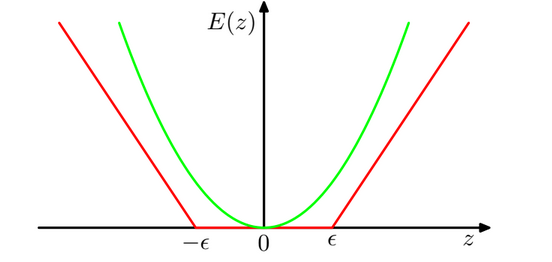
\includegraphics[width=15cm]{images/Kernel Methods/ksvm.png}
    \label{fig:ksvm}
    \caption{error function for linear regression that makes the kernel sparse.}
\end{figure}

Problem: it is not differentiable, so it is difficult to solve.

We can the introduce \textit{slack variables} $\xi_{n}^{+}, \xi_{n}^{-} \geq 0$:
\begin{equation}
\label{eq:ksvm_condition1}
    \begin{multlined}
        t_{n} \leq y_{n} + \epsilon + \xi_{n}^{+} \\
        t_{n} \leq y_{n} - \epsilon - \xi_{n}^{-}
    \end{multlined}
\end{equation}
Points that are into the $\epsilon$-tube $y_{n} - \epsilon \leq t_{n} \leq t_{n} + \epsilon \Rightarrow \xi_{n} = 0$
\begin{equation}
\label{eq:ksvm_condition2}
    \begin{multlined}
        \xi_{n}^{+} > 0 \Rightarrow y_{n} + \epsilon \\
        \xi_{n}^{-} > 0 \Rightarrow y_{n} - \epsilon
    \end{multlined}
\end{equation}
with $y_{n} = t(x_{n}, w)$. \\
The loss function can be rewritten as:
\begin{equation}
    J(w) = C\sum_{n=0}^{N}(\xi^{+}_{n} + \xi^{-}_{n}) + \frac{1}{2}||w||^{2}
\end{equation}
subject to \ref{eq:ksvm_condition1} and \ref{eq:ksvm_condition2}.\\
This is a standard quadratic program (QP), can be “easily” solved.
The Lagrangian problem is:
\begin{equation}
    \Tilde{L}(a, a') = \dots \sum_{n=1}^{N}\sum_{m=1}^{N}a_{n}a_{m}\dots k(x_{\Tilde{n}}, x_{m}) \dots
\end{equation}
from which we compute $\hat{a}_{n}$, $\hat{a}_{m}'$ (sparse values, most of them are zero) and
\begin{equation}
    \hat{w}_{0} = t_{n} - \epsilon - \sum_{m=1}^{N}(\hat{a}_{m} - \hat{a}_{m}')k(x_{n},x_{m})
\end{equation}
for some data point $n$ such that $0 < a_{n} < C$. \\
The \textbf{prediction} is:
\begin{equation}
    y(x) = \sum_{n=1}^{N}(\hat{a}_{\Tilde{n}} - \hat{a}_{n})'k(x, x_{n}) + \hat{w}_{0}
\end{equation}
From Karush-Kuhn-Tucker (KKT) condition, \textbf{support vectors} contribute to predictions
\[\hat{a}_{n} > 0 \Rightarrow \epsilon + \xi_{n} + y_{n} - t_{n} = 0\]
data point lies on or above upper boundary of the $\epsilon-tube$, while
\[\hat{a}_{n}' > 0 \Rightarrow \epsilon + \xi_{n} - y_{n} + t_{n} = 0\]
data point lies on or below lower boundary of the $\epsilon$-tube. All other datapoints inside the $\epsilon$-tube have $\hat{a}_{n} = 0$ and  $\hat{a}_{n}' = 0$ and thus do not contribute to prediction.
\begin{figure}[H]
    \centering
    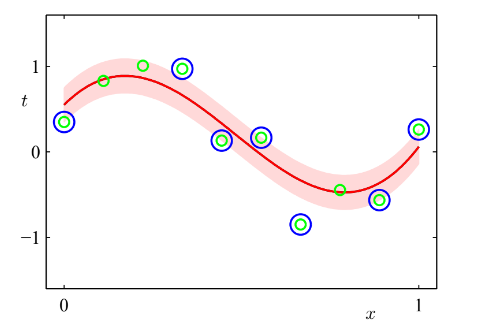
\includegraphics[width=15cm]{images/Kernel Methods/epsilon_tube.png}
    \label{fig:epsilon_tube}
\end{figure}